\documentclass[11pt]{article}

\usepackage[margin=1in]{geometry}
\usepackage{graphicx}
\usepackage{booktabs}
\usepackage{amsmath}
\usepackage{amssymb}
\usepackage{hyperref}
\usepackage{xcolor}
\usepackage{tikz}
\usetikzlibrary{arrows.meta, positioning, calc, fit}

\title{\textbf{zklora: Verifiable Multi-Party Inference for Evaluating Private LoRA Weights}}
\author{Anonymous Authors}
\date{\today}

\begin{document}

\maketitle

\begin{abstract}
In decentralized computing environments, one party may wish to fine-tune a publicly available base model with Low-Rank Adaptation (LoRA) but keep those adapter weights private, while another party wants to evaluate performance on new data. 
We introduce \texttt{zklora}, a library designed to help the \emph{Base Model User} \emph{verifiably assess} the quality of a private LoRA module for a target task---for instance, to run a validation experiment without directly accessing the private weights. 
By adopting a multi-party inference approach and generating \emph{verifiable computations}, \texttt{zklora} enables the \emph{Base Model User} to confirm that remote LoRA computations are correct, all without seeing the private weights themselves. 
We demonstrate the feasibility of \texttt{zklora} via benchmark experiments, showing that our approach remains computationally viable across various model sizes, with notably fast verification times.
\end{abstract}

%------------------------------------------
% 4. INTRODUCTION
%------------------------------------------
\section{Introduction}

Large Language Models (LLMs) excel at a variety of tasks but come with significant computational and storage costs \cite{brown2020language, devlin2018bert}. 
Low-Rank Adaptation (LoRA) \cite{hu2021lora} addresses these costs by introducing a small number of trainable parameters into the model, drastically reducing memory overhead for fine-tuning \cite{ding2022delta}. 

When two entities, a \emph{LoRA Owner} and a \emph{Base Model User}, collaborate on a shared LLM, they may have conflicting constraints. The \emph{LoRA Owner} wants to keep custom LoRA weights private (e.g., for competitive or regulatory reasons), while the \emph{Base Model User} wants to \emph{test} or \emph{validate} these LoRA weights on a target task before deciding whether to deploy them at scale. Under normal circumstances, either the LoRA must be fully shared (sacrificing privacy), or the Base Model User must trust the LoRA Owner’s claims about performance with little evidence.

\texttt{zklora} bridges this gap by orchestrating multi-party inference: the base model user remains in control of the main layers, whereas the LoRA Owner privately applies LoRA transformations. The user obtains a zero-knowledge proof demonstrating that the LoRA transformations are indeed correct, thus verifying the final performance metrics. Once satisfied that the LoRA weights meet their needs, the Base Model User can incorporate them at scale through whatever inference arrangement they prefer.

%------------------------------------------
% 1. PRELIMINARY RESULTS
%------------------------------------------
\section{Preliminary Results}

We benchmarked \texttt{zklora} by measuring the creation and verification times for our verifiable computations across multiple base models and private LoRA configurations. For each model, we computed a forward pass for a batch of 3 items with sequence length 5. 
Each experiment simulates the workflow where the \emph{Base Model User} uses local data to evaluate the base model + LoRA combination, requesting remote LoRA computations from the \emph{LoRA Owner}. 
We report total and average proof-generation times (\texttt{total\_prove}, \texttt{avg\_prove}) and verification times (\texttt{total\_verify}, \texttt{avg\_verify}), as well as relevant model parameters.

\begin{table}[ht]
    \centering
    \small
    \begin{tabular}{l c c c c c c c}
    \toprule
    \textbf{base\_model} & \textbf{\#lora} & \textbf{total\_params} & \textbf{avg\_params} & \textbf{total\_prove} & \textbf{avg\_prove} & \textbf{total\_verify} & \textbf{avg\_verify} \\
    \midrule
distilgpt2 & 24 & 589824 & 24576.0 & 759.33 & 31.64 & 16.56 & 0.69 \\
gpt2 & 48 & 2359296 & 49152.0 & 1675.58 & 34.91 & 32.79 & 0.68 \\
Llama-3.2-1B & 32 & 851968 & 26624.0 & 991.93 & 31.00 & 24.91 & 0.78 \\
Llama-3.3-70B-Instr. & 80 & 11796480 & 147456.0 & 3749.76 & 46.87 & 123.11 & 1.54 \\
Llama-3.1-8B-Instr. & 32 & 5242880 & 163840.0 & 1527.40 & 47.73 & 35.79 & 1.12 \\
Mixtral-8x7B-Instr. & 32 & 10485760 & 327680.0 & 2357.61 & 73.68 & 44.30 & 1.38 \\
    \bottomrule
    \end{tabular}
    \caption{Benchmark results for \texttt{zklora} showing multi-party inference overhead on various model + LoRA combinations. Times are in seconds.}
    \label{tab:results}
\end{table}

Notably, although proof-generation times can grow with model size, verification remains comparatively fast (e.g., an average of around 1--2 seconds per proof even for 70B-scale models). This result demonstrates that \texttt{zklora} allows frequent correctness checks without excessive overhead, which is crucial for real-world “trial runs.” In larger-scale usage scenarios, once trust in the LoRA module is established, \texttt{zklora} may no longer be needed.

%------------------------------------------
% 2. MULTI-PARTY INFERENCE METHOD
%------------------------------------------
\section{Multi-Party Inference: zklora for Verifiable Evaluation}

Our aim is to enable the \emph{Base Model User} to run a \emph{validation experiment} on their local data, incorporating the private LoRA module from the \emph{LoRA Owner}. The Base Model User can measure task performance (e.g., cross-entropy loss, accuracy) to decide whether the LoRA meets performance requirements. 

Figure~\ref{fig:toy-mlp-lora} illustrates a simple scenario in which:

\begin{enumerate}
    \item \textbf{Base Model Forward Pass (Base Model User).}
    The \emph{Base Model User} runs layers without LoRA parameters locally, generating partial activations.

    \item \textbf{Forward to LoRA Adapter (Base Model User).}
    Whenever the next layer includes a LoRA transform, the \emph{Base Model User} sends these partial activations to the \emph{LoRA Owner}, who holds the private LoRA module.

    \item \textbf{LoRA Computation \& Proof Generation (LoRA Owner).}
    The \emph{LoRA Owner} applies the LoRA transformation to the activations and returns the updated activations alongside a \emph{cryptographic proof} of correctness.

    \item \textbf{Resuming the Forward Pass (Base Model User).}
    The \emph{Base Model User} injects the updated activations back into the local model state and continues the forward pass. 

    \item \textbf{Verification \& Validation (Base Model User).}
    The \emph{Base Model User} verifies the LoRA proof. If valid, the outputs from the combined base + LoRA model are guaranteed to match the LoRA Owner’s claimed computation. The Base Model User can now measure final metrics (loss, accuracy, etc.) to assess \emph{quality} on the target task.
\end{enumerate}

\begin{figure}[ht]
\centering
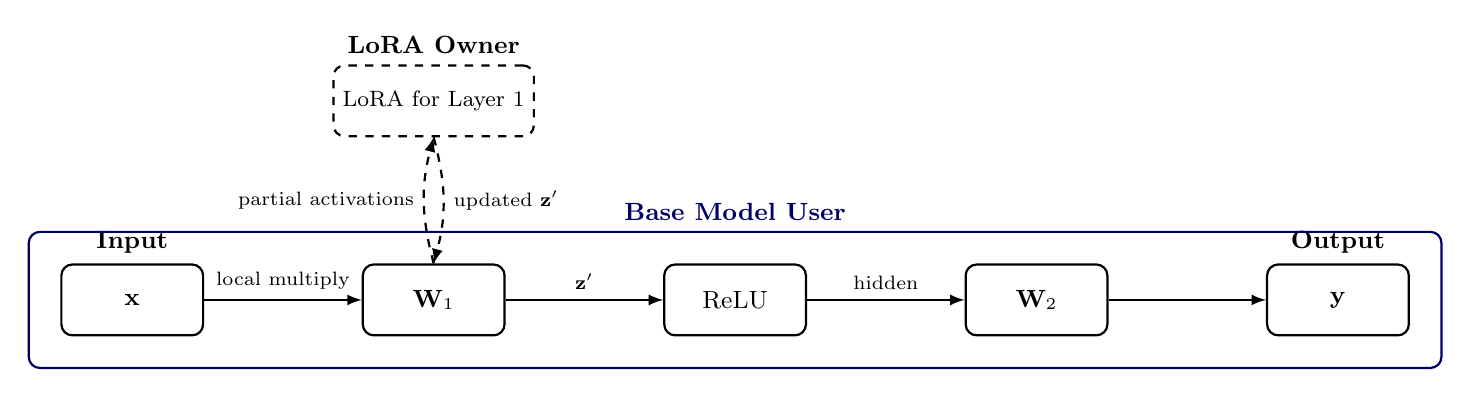
\begin{tikzpicture}[
    font=\small,
    >=latex,
    thick,
    block/.style={
      draw,
      rounded corners,
      align=center,
      minimum width=1.8cm,
      minimum height=0.9cm
    },
    dashedblock/.style={
      draw,
      dashed,
      rounded corners,
      align=center,
      font=\footnotesize,
      fill=white,
      minimum width=1.8cm,
      minimum height=0.9cm
    },
    arrow/.style={->, thick},
    node distance=2.0cm
]

\node[block, label=above:\textbf{Input}] (input) {$\mathbf{x}$};
\node[block, right=2.0cm of input] (W1) {$\mathbf{W}_1$};
\node[dashedblock, above=1.6cm of W1, label=above:\textbf{LoRA Owner}] (LoRA) {LoRA for Layer 1};
\node[block, right=2.0cm of W1] (act) {ReLU};
\node[block, right=2.0cm of act] (W2) {$\mathbf{W}_2$};
\node[block, label=above:\textbf{Output}, right=2.0cm of W2] (output) {$\mathbf{y}$};

\draw[->] (input) -- node[above, font=\scriptsize]{local multiply} (W1);
\draw[->, dashed] (W1.north) to[bend left=15] node[left, font=\scriptsize]{partial activations} (LoRA.south);
\draw[->, dashed] (LoRA.south) to[bend left=15] node[right, font=\scriptsize]{updated $\mathbf{z}'$} (W1.north);
\draw[->] (W1) -- node[above, font=\scriptsize]{$\mathbf{z}'$} (act);
\draw[->] (act) -- node[above, font=\scriptsize]{hidden} (W2);
\draw[->] (W2) -- (output);

\node[draw, rounded corners, thick, color=blue!40!black,
      fit=(input)(W1)(act)(W2)(output),
      label={[font=\small, color=blue!40!black]above:\textbf{Base Model User}},
      inner sep=0.4cm
] (baseModelFit) {};
\end{tikzpicture}
\caption{A simplified 2-layer MLP with LoRA on the first layer. The Base Model User (blue box) runs most computations locally but calls the LoRA Owner (dashed box) to update partial activations. After verifying correctness, the Base Model User can measure final metrics to decide whether to adopt the private LoRA more extensively.}
\label{fig:toy-mlp-lora}
\end{figure}

%------------------------------------------
% 3. HOW WE GENERATE THE ZERO-KNOWLEDGE PROOF
%------------------------------------------
\section{Generating the Zero-Knowledge Proof}

A central piece of our methodology is producing a cryptographic proof that the LoRA transformations were correctly computed—without ever disclosing the LoRA parameters themselves. We outline the proof-generation process below, referencing the flow in the accompanying code. For simplicity, we assume the LoRA Owner has already exported the LoRA-modified layer(s) as an ONNX model and that intermediate activations are saved in a JSON file. Each pairing of “model file” and “JSON input data” yields a distinct proof.

\subsection{Preparing Model, Inputs, and Circuit}
\paragraph{Circuit and ONNX File.}
The LoRA Owner provides an ONNX model that includes the relevant LoRA weights. We then compile this model into a zero-knowledge friendly circuit format. This step:
\begin{itemize}
    \item Parses the graph structure from the ONNX file.
    \item Determines how many constraints or “gates” are needed.
    \item Produces a circuit representation that can be used for further proof-generation steps.
\end{itemize}

\paragraph{Input Activations (JSON).}
When the \emph{Base Model User} runs the partial forward pass locally, the intermediate activations for that partial pass are recorded in a JSON file. This JSON effectively captures the inbound tensor(s) that will go through the remote LoRA layers.

\subsection{Generating Setup and Keys}
\paragraph{Settings and Keys.}
To make the cryptographic proof work, the system needs:
\begin{itemize}
    \item \textbf{Settings File:} Summarizes the circuit’s structure (e.g., log rows, public vs. private parameters). 
    \item \textbf{Proving/Verification Keys (PK/VK):} Analogous to a public-private key system, enabling one party to prove a statement and another to verify.
\end{itemize}
We produce these keys from the compiled circuit. If the protocol also requires a structured reference string (SRS), we generate that as well. This SRS encapsulates certain group elements or domain parameters for polynomial commitments, usually saved in a file.

\subsection{Generating the Witness}
\paragraph{Witness Creation.}
With the circuit in place, we feed the JSON data for intermediate activations into the compiled circuit. This step:
\begin{itemize}
    \item Performs the actual forward pass inside the circuit, substituting the LoRA parameters from the ONNX file.
    \item Produces a “witness file,” which is a low-level representation of all wire values in the circuit.
\end{itemize}
In practice, this might be asynchronous or batched, ensuring large inputs can be processed efficiently.

\subsection{Proof Generation}
\paragraph{Prove.}
Once we have:
\begin{itemize}
    \item The circuit representation.
    \item The proving key (PK).
    \item The witness file.
\end{itemize}
we invoke a “prove” routine that executes polynomial commitment schemes and solves the constraint system. This yields a standalone proof file that can be shared with the \emph{Base Model User}.

\paragraph{Result.}
The final proof cryptographically certifies that the LoRA Owner used the declared ONNX model and input JSON to compute the updated activations \emph{exactly} as claimed, with no tampering or hidden changes.

\subsection{Proof Verification}
\paragraph{Checking the Proof.}
The \emph{Base Model User}, upon receiving the proof, uses:
\begin{itemize}
    \item The verification key (VK).
    \item The structured reference string (SRS).
    \item The proof file.
\end{itemize}
A single verification call then confirms or denies the proof’s correctness. If correct, it implies that the LoRA transformations were faithfully applied.

\paragraph{Timing.}
In our benchmarks, this verification step is typically on the order of 1–2 seconds, even for large models, as shown in Table~\ref{tab:results}. The minimal overhead of verification makes \texttt{zklora} feasible for continuous or repeated “trial runs” to confirm LoRA quality.



%------------------------------------------
% 5. RELATED WORK
%------------------------------------------
\section{Related Work}

\subsection{Low-Rank Adaptation}
LoRA \cite{hu2021lora} has emerged as a popular way to efficiently fine-tune LLMs by injecting small, low-rank matrices into specific layers. This approach scales well, requiring less GPU memory than full fine-tuning. Various frameworks build on LoRA for GPT-2, GPT-Neo, LLaMA, and others \cite{ding2022delta}. By confining most updated parameters to low-rank adapter matrices, LoRA drastically reduces memory overhead during fine-tuning.

\subsection{Incrementally Verifiable Computation}
Valiant~\cite{valiant2008incrementally} introduced the notion of Incrementally Verifiable Computation (IVC), which offers updatable, compact proofs of correctness over multi-step computations. Follow-up work \cite{kothapalli2022nova, kothapalli2024hypernova} refines these ideas, leveraging folding schemes and zero-knowledge properties to enable scaling of verifiable computations. While prior research has investigated IVC for inference or specialized tasks, \texttt{zklora} adapts such cryptographic proof techniques for verifying private LoRA transformations in multi-party inference.

%------------------------------------------
% 6. CONCLUSION
%------------------------------------------
\section{Conclusion}

\texttt{zklora} enables a \emph{Base Model User} to verify the quality of a private LoRA module without revealing the LoRA weights. Our benchmarks show that proof generation remains feasible for multiple model sizes, and verification overhead is small enough to allow iterative experiments. This design provides strong assurances of correctness while preserving LoRA privacy. Future directions include optimizing circuit compilation, supporting multi-owner LoRA composition, and investigating broader multi-party computation frameworks that incorporate private data alongside private model parameters.

\bibliographystyle{plain}
\bibliography{references}

\end{document}
